\subsection{Scenarios} \comment[id=K]{Add parameter notation when writing this.}
\label{subsec:appendix_scenarios}



\begin{figure}[ht] % Work Scenarios
  \centering
  \begin{subfigure}[b]{.49\textwidth}
    \centering
    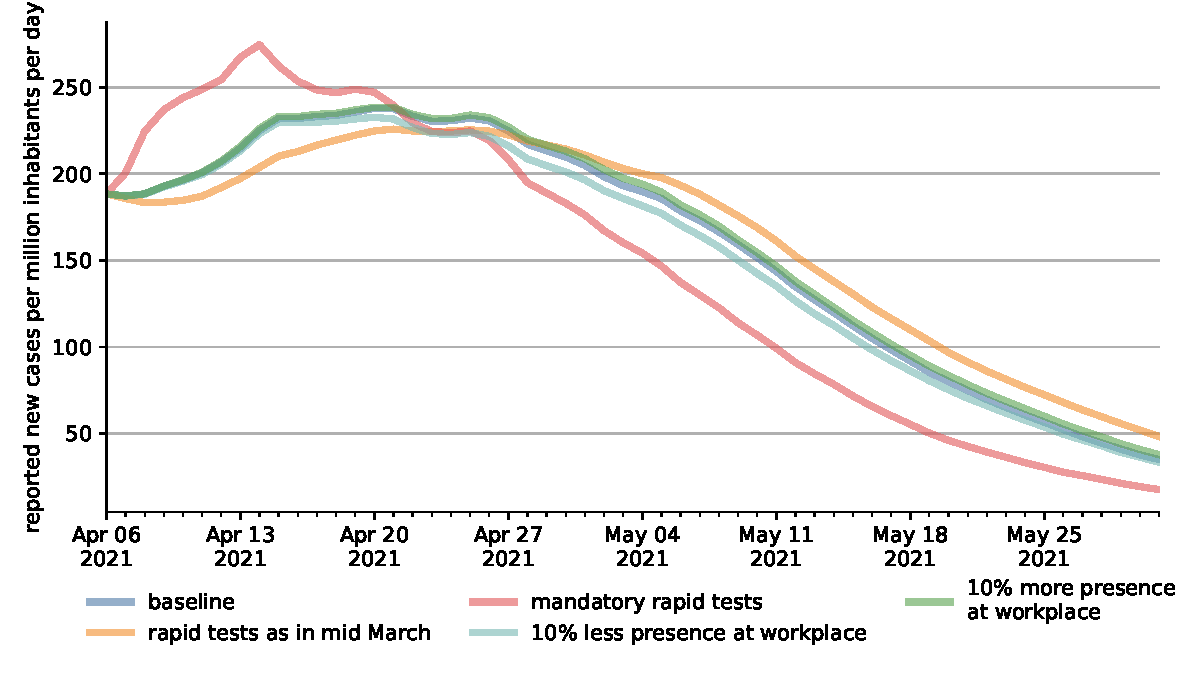
\includegraphics[width=0.9 \textwidth]{figures/results/figures/scenario_comparisons/new_work_scenarios/full_new_known_case}
    \caption{Reported Cases}
    \label{fig:work_scenarios_new_known_case}
  \end{subfigure}
  \hfill
  \begin{subfigure}[b]{.49\textwidth}
    \centering
    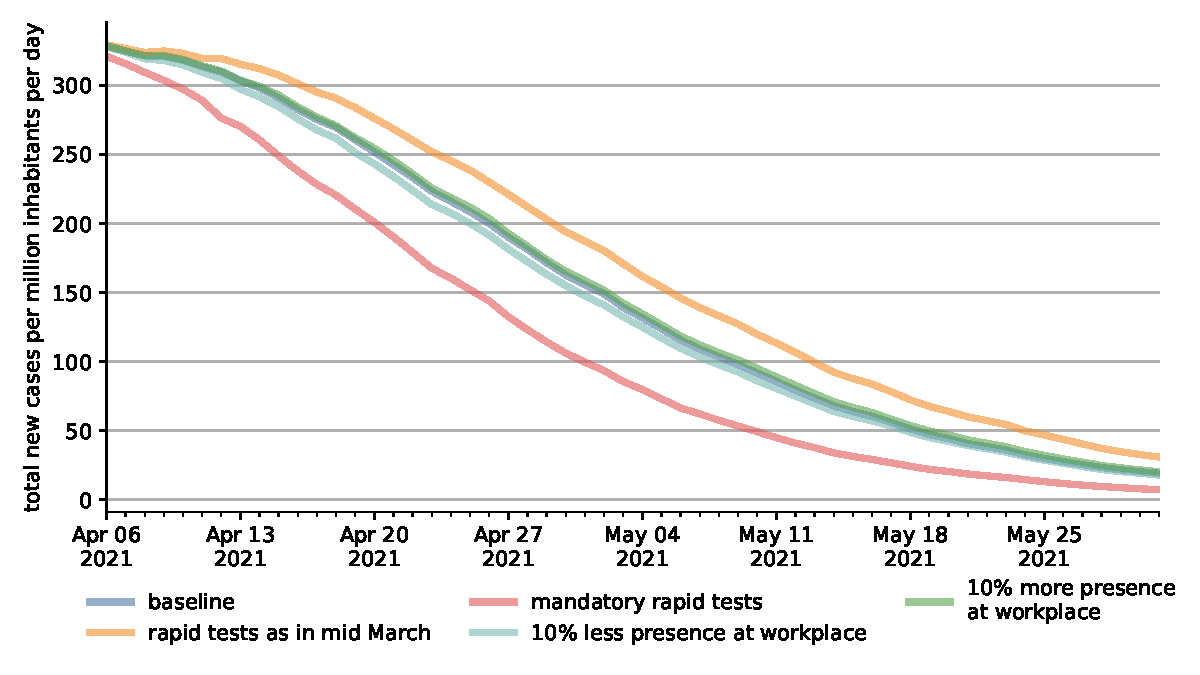
\includegraphics[width=0.9 \textwidth]{figures/results/figures/scenario_comparisons/new_work_scenarios/full_newly_infected}
    \caption{Total Cases}
    \label{fig:work_scenarios_newly_infected}
  \end{subfigure}
  \caption{The Effect of Different Work Scenarios on Reported and Total Cases}
  \label{fig:work_scenarios_detailed}
  \floatfoot{\noindent \textit{Note:} The figure shows the development of cases after the
  policy changes took place at Easter until the end of our simulation period (end of
  May). We vary the share of workers that work from home and how many tests are performed
  at work relative to our baseline scenario. Making it mandatory to test all employees
  that do not work from home markedly reduces cases -- even when only assuming 95\%
  compliance on both the employer and the employee side. As before, the observed cases
  can be misleading because more testing leads to more detected cases. It takes two to
  three weeks for the reduction in new infections effect to dominate the increased
  detection effect. Furthermore, the two opposing effects lead to a smaller effect size
  than is actually the case.}
\end{figure}

 \comment[id=K]{Regarding figure \ref{fig:work_scenarios_detailed}: Look up numbers and
 add them to the description.}


\begin{figure}[ht] % School Scenarios
  \centering
  \begin{subfigure}[b]{.49\textwidth}
    \centering
    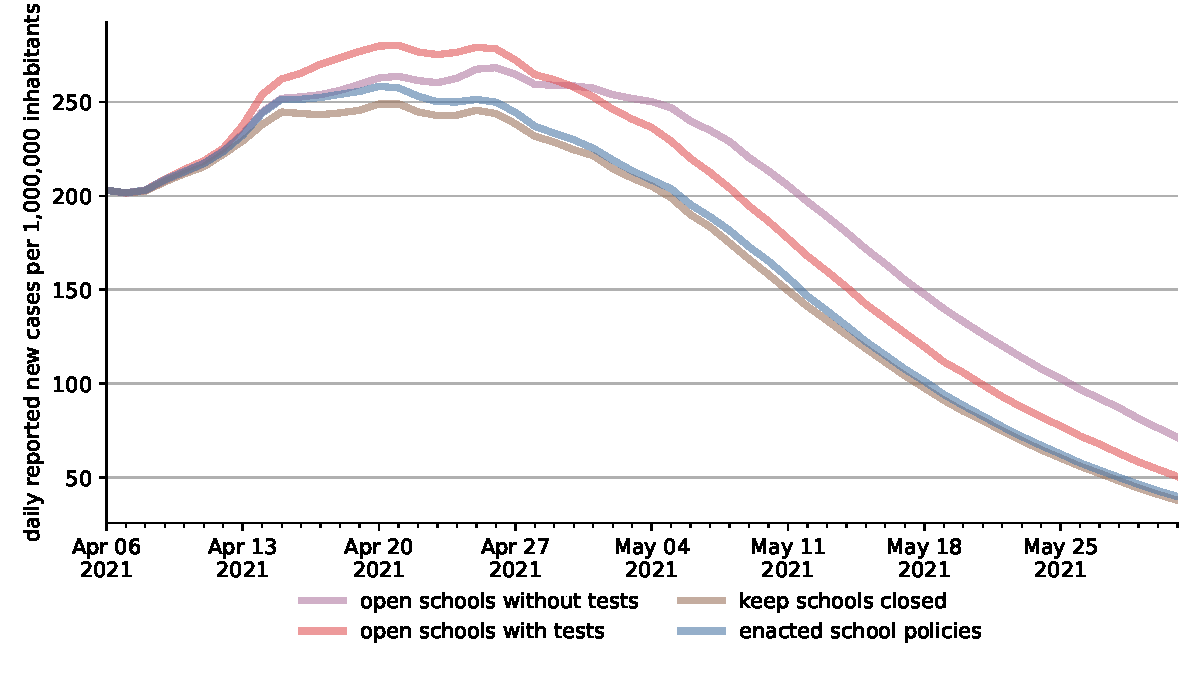
\includegraphics[width=0.9 \textwidth]{figures/results/figures/scenario_comparisons/school_scenarios/full_new_known_case}
    \caption{Reported Cases}
    \label{fig:school_scenarios_new_known_case}
  \end{subfigure}%
  \hfill
  \begin{subfigure}[b]{.49\textwidth}
    \centering
    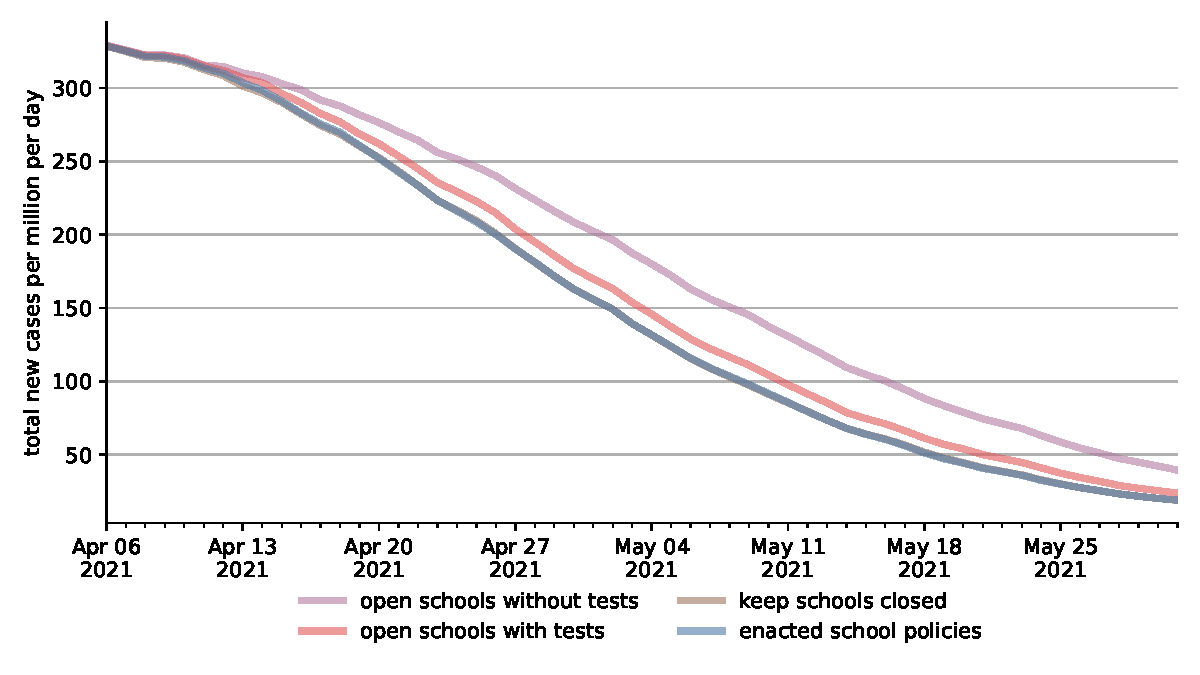
\includegraphics[width=0.9 \textwidth]{figures/results/figures/scenario_comparisons/school_scenarios/full_newly_infected}
    \caption{Total Cases}
    \label{fig:school_scenarios_newly_infected}
  \end{subfigure}
  \caption{The Effect of Different School Scenarios on Reported and Total Cases}
  \label{fig:school_scenarios_detailed}
  \floatfoot{\noindent \textit{Note:} The figure shows the development of cases after the
   policy changes took place at Easter until the end of our simulation period (end of
   May). Apart from the enacted school policies as our baseline we simulate how cases
   would have developed if schools had been closed completely as the strictest possible
   counterfactual scenario and two opening models: One where schools open normally (with
   hygiene measures) without any testing in the education sector and one where schools
   open normally but testing shares develop as in the baseline scenario. Our simulations
   suggest that the enacted policies were as effective as keeping schools closed. Opening
   schools with the testing schemes that were in place after Easter would have had a
   small effect on the overall incidence. However, this is mainly due to the stringent
   testing that was in place in schools by that time. Had schools opened without testing
   requirements the total incidence would have been up to 50 points higher, though this
   would have been less visible in the reported cases.}
\end{figure}

 \comment[id=K]{Regarding figure \ref{fig:school_scenarios_detailed}: Look up numbers and
 add them to the description.}


\begin{figure}[ht] % Random Rapid Tests
  \centering
  \begin{subfigure}[b]{.49\textwidth}
    \centering
    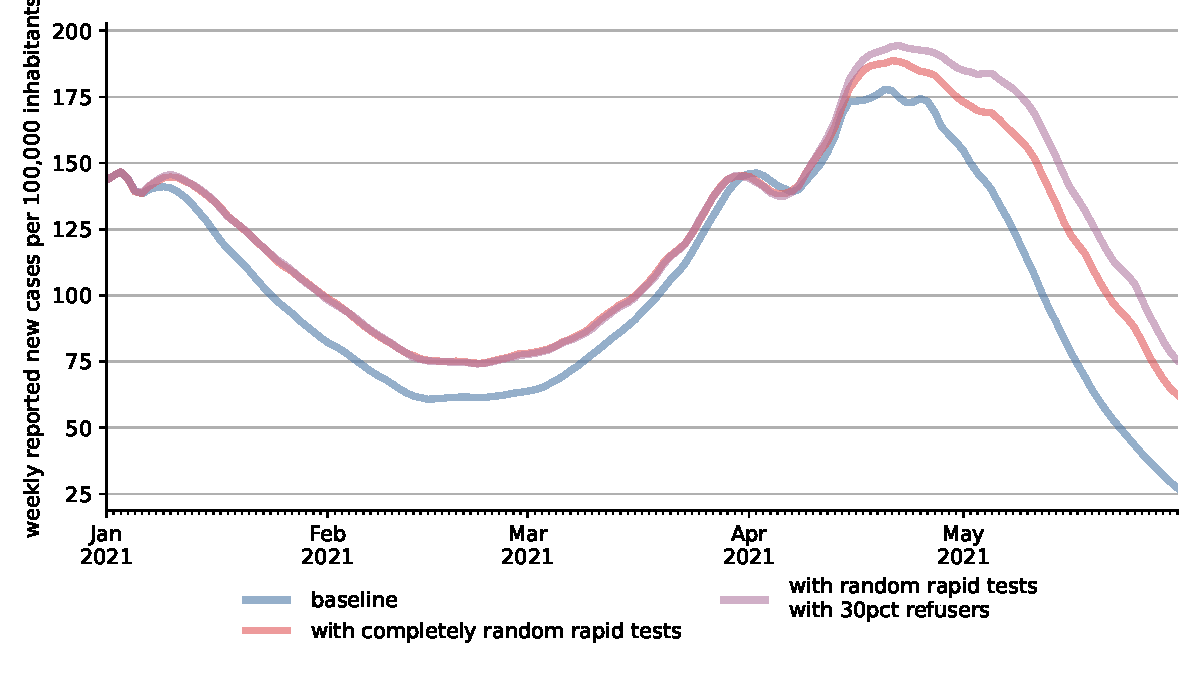
\includegraphics[width=0.9 \textwidth]{figures/results/figures/scenario_comparisons/random_rapid_tests_vs_baseline/full_new_known_case}
    \caption{Reported Cases}
    \label{fig:random_rapid_tests_new_known_case}
  \end{subfigure}%
  \hfill
  \begin{subfigure}[b]{.49\textwidth}
    \centering
    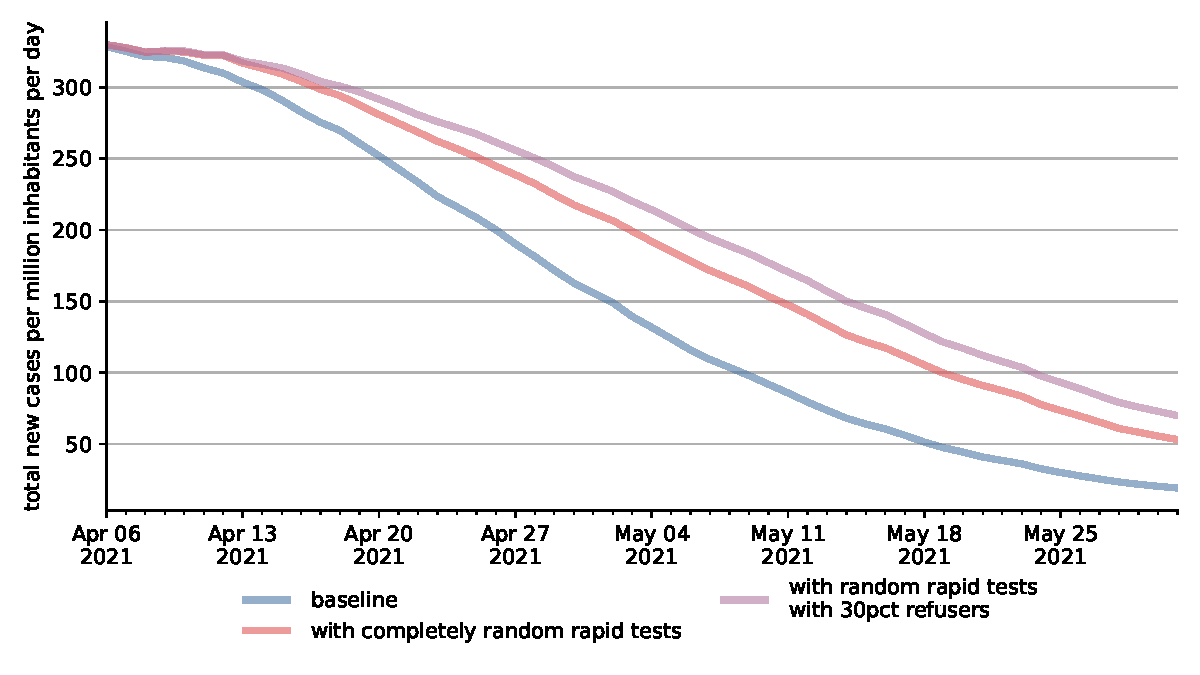
\includegraphics[width=0.9 \textwidth]{figures/results/figures/scenario_comparisons/random_rapid_tests_vs_baseline/full_newly_infected}
    \caption{Total Cases}
    \label{fig:random_rapid_tests_newly_infected}
  \end{subfigure}
  \caption{The Role of Targeted and Compliance Driven Rapid Test Demand}
  \label{fig:random_rapid_tests_detailed}
  \floatfoot{\noindent \textit{Note:} \textcolor{red}{To be written}}
\end{figure}

 \comment[id=K]{Describe that random tests are more effective at detecting cases and that
 explains the bump in the random test scenario detection in the beginning. However, cases
 fall immediately more in the non-random scenario because the targeted demand for tests
 by household members leads to a much more efficient interruption of infection chains
 because we catch the household members very early in their infectious period.}

 \comment[id=K]{Write that at the end of our simulation period nearly everyone in the
 educ sector did rapid tests because they are mandatory but still 40-50\% refusers in the
 work and private sector}

\FloatBarrier
